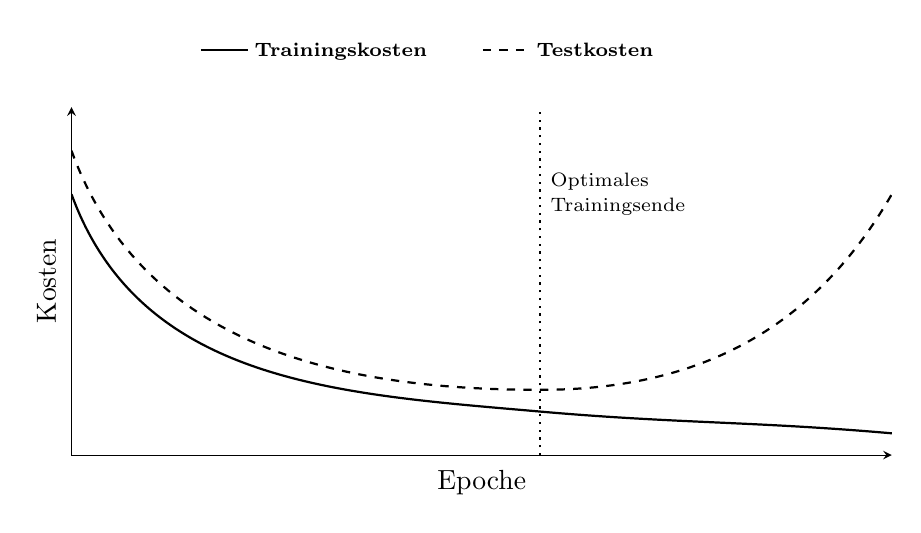
\begin{tikzpicture}[
    curve/.style={
        thick,
        domain=0:14,
    },
]

    \begin{axis}[
        width=12cm,
        height=6cm,
        axis x line=center,
        axis y line=center,
        xmin=0, xmax=14,
        ymin=0, ymax=8,
        xlabel=Epoche, xtick style={draw=none}, xtick=\empty,
        ylabel=Kosten, ytick style={draw=none}, ytick=\empty,
        xlabel near ticks,
        ylabel near ticks,
        legend columns=-1,
        legend style={
            at={(0.5,1.1)},
            anchor=south,
            draw=none,
            font=\scriptsize\bfseries,
            text width=8em,
            text height=1.5ex,
            text depth=.5ex,
        },
    ]
        \draw[curve]
            (axis cs:0,6) to[out=-70,in=175]
            (axis cs:8,1) to[out=-5,in=175]
            (axis cs:14,0.5);

        \draw[curve, dashed]
            (axis cs:0,7) to[out=-70,in=180]
            (axis cs:8,1.5) to[out=0,in=240]
            (axis cs:14,6);

        \addlegendimage{curve}
        \addlegendentry{Trainingskosten}
        \addlegendimage{curve,dashed}
        \addlegendentry{Testkosten}

        \draw[dotted, thick] (axis cs:8,0) -- node[near end,right,text width=5em]{\scriptsize{Optimales\\[-1ex]Trainingsende}} (axis cs:8,8);
    \end{axis}
\end{tikzpicture}
